%% Aide-mémoire
\documentclass[10pt, french]{article}
%% -----------------------------
%% Préambule
%% -----------------------------
\usepackage{xcolor}
\usepackage{bbding}
\usepackage{pifont}
\usepackage{multido}
\def\cours{Modern Actuarial Statistics}
\def\sigle{MAS-I}
\def\session{Avril 2019}
\def\auteur{Nicholas Langevin}
\def\BackgroundColor{white}
% \definecolor{section_color}{rgb}{0.1,0.1,1}
\def\SubSectionColor{blue!30!black}
% !TEX encoding = UTF-8 Unicode
% LaTeX Preamble
% Author : Gabriel Crépeault-Cauchon

% HOW-TO : copy-paste this file in the same directory as your .tex file, and add in your preamble the next command right after you have specified your documentclass : 
% \input{preamble-cheatsht.tex}
% ---------------------------------------------
% ---------------------------------------------

%% -----------------------------
%% Encoding packages
%% -----------------------------
\usepackage[utf8]{inputenc}
\usepackage[T1]{fontenc}
\usepackage{babel}
\usepackage{lmodern}

%% -----------------------------
%% Variable definition
%% -----------------------------


\def\session{Automne 2018}
\def\auteur{Gabriel Crépeault-Cauchon // Nicholas Langevin}
\def\BackgroundColor{white}


%% -----------------------------
%% Margin and layout
%% -----------------------------
% Determine the margin for cheatsheet
\usepackage[landscape, hmargin=1cm, vmargin=1.7cm]{geometry}
\usepackage{multicol}

% Remove automatic indentation after section/subsection title.
\setlength{\parindent}{0cm}

% Save space in cheatsheet by removing space between align environment and normal text.
\usepackage{etoolbox}
\newcommand{\zerodisplayskips}{%
  \setlength{\abovedisplayskip}{0pt}%
  \setlength{\belowdisplayskip}{0pt}%
  \setlength{\abovedisplayshortskip}{0pt}%
  \setlength{\belowdisplayshortskip}{0pt}}
\appto{\normalsize}{\zerodisplayskips}
\appto{\small}{\zerodisplayskips}
\appto{\footnotesize}{\zerodisplayskips}

%% -----------------------------
%% URL and links
%% -----------------------------
\usepackage{hyperref}
\hypersetup{colorlinks = true, urlcolor = gray!70!white, linkcolor = black}

%% -----------------------------
%% Document policy (uncomment only one)
%% -----------------------------
%	\usepackage{concrete}
	\usepackage{mathpazo}
%	\usepackage{frcursive} %% permet d'écrire en lettres attachées
%	\usepackage{aeguill}
%	\usepackage{mathptmx}
%	\usepackage{fourier} 

%% -----------------------------
%% Math configuration
%% -----------------------------
\usepackage[fleqn]{amsmath}
\usepackage{amsthm,amssymb,latexsym,amsfonts}
\usepackage{empheq}
\usepackage{numprint}

% Mathematics shortcut
\newcommand{\reels}{\mathbb{R}}
\newcommand{\entiers}{\mathbb{Z}}
\newcommand{\naturels}{\mathbb{N}}
\newcommand{\eval}{\biggr \rvert}
\usepackage{cancel}
\newcommand{\derivee}[1]{\frac{\partial}{\partial #1}}
\newcommand{\prob}[1]{\Pr \left( #1 \right)}
\newcommand{\esp}[1]{\mathrm{E} \left[ #1 \right]}
\newcommand{\variance}[1]{\mathrm{Var} \left( #1 \right)}
\newcommand{\covar}[1]{\mathrm{Cov} \left( #1 \right)}
\newcommand{\laplace}{\mathcal{L}}

% To indicate equation number on a specific line in align environment
\newcommand\numberthis{\addtocounter{equation}{1}\tag{\theequation}}

% Actuarial notation package
\usepackage{actuarialsymbol}
\usepackage{actuarialangle}

% Matricial anotation for math symbols (\bm{•})
\usepackage{bm}
% matricial notation variable (bold style)
\newcommand{\matr}[1]{\mathbf{#1}}



%% -----------------------------
%% tcolorbox configuration
%% -----------------------------
\usepackage{tcolorbox}
\tcbuselibrary{xparse}
\tcbuselibrary{breakable}

%% Définition boite pour définition
\DeclareTColorBox{definition}{ o }% #1 parameter
{colframe=blue!60!green,colback=blue!5!white, % color of the box
breakable, pad at break*=0mm, % to split the box
title = {#1},
after title = {\large \hfill \faBook}
}

%% -----------------------------
%% Graphics and pictures
%% -----------------------------
\usepackage{graphicx}
\usepackage{pict2e}

%% -----------------------------
%% insert pdf pages into document
%% -----------------------------
\usepackage{pdfpages}

%% -----------------------------
%% Color configuration
%% -----------------------------
\usepackage{color, soulutf8, colortbl}


% New color definition
% Source : http://latexcolor.com


% usefull shortcut for colored text
\newcommand{\orange}{\textcolor{orange}}
\newcommand{\red}{\textcolor{red}}
\newcommand{\cyan}{\textcolor{cyan}}
\newcommand{\blue}{\textcolor{blue}}
\newcommand{\green}{\textcolor{green}}
\newcommand{\purple}{\textcolor{magenta}}
\newcommand{\yellow}{\textcolor{yellow}}


%% -----------------------------
%% Enumerate environment configuration
%% -----------------------------
% Custum enumerate & itemize Package
\usepackage{enumitem}
% French Setup for itemize function
\frenchbsetup{StandardItemLabels=true}
% Change default label for itemize
\renewcommand{\labelitemi}{\faAngleRight}

%% -----------------------------
%% Tabular column type configuration
%% -----------------------------
\newcolumntype{C}{>{$}c<{$}} % math-mode version of "l" column type
\newcolumntype{L}{>{$}l<{$}} % math-mode version of "l" column type
\newcolumntype{R}{>{$}r<{$}} % math-mode version of "l" column type
\newcolumntype{f}{>{\columncolor{green!20!white}}p{1cm}}
% configuration to force a line break within a single cell
\usepackage{makecell}



%% -----------------------------
%% Fontawesome for special symbols
%% -----------------------------
\usepackage{fontawesome}

%% -----------------------------
%% Section Font customization
%% -----------------------------
\usepackage{sectsty}
\sectionfont{\color{\SectionColor}}
\subsectionfont{\color{\SubSectionColor}}

%% -----------------------------
%% Footer/Header Customization
%% -----------------------------
\usepackage{lastpage}
\usepackage{fancyhdr}
\pagestyle{fancy}
% Header
\fancyhead{} 	% Reset
\fancyhead[L]{Aide-mémoire pour~ \cours ~(\textbf{\sigle})}
\fancyhead[R]{\auteur}

% Footer
\fancyfoot{}		% Reset
\fancyfoot[R]{\thepage ~de~ \pageref{LastPage}}
\fancyfoot[L]{\href{https://github.com/gabrielcrepeault/latex-template}{\faGithub \ gabrielcrepeault/latex-template}}

% page background color
\pagecolor{\BackgroundColor}






%% END OF PREAMBLE
% ---------------------------------------------
% ---------------------------------------------
\title{MAS-1 \\ Study Review}
\author{Nicholas Langevin}
%% -----------------------------
%% Début du document
%% -----------------------------
\begin{document}

\maketitle 
\vspace{50px}
\begin{center}
\begin{minipage}[c]{7.5cm}
    \begin{itemize}
        \LARGE
        \item[\color{magenta}\ding{235}] Probability Review 
        \item[\color{brown}  \ding{235}] \hyperref[Stochastic Processes]{Stochastic Processes} 
        \item[\color{purple} \ding{235}] Life Contingencies
        \item[\color{orange} \ding{235}] Simulation
        \item[\color{red}    \ding{235}] Statistics
        \item[\color{blue}   \ding{235}] Extended Linear Model
        \item[\color{green}  \ding{235}] Time Series      
    \end{itemize}
\end{minipage}
\end{center}
\newpage

\small
\begin{multicols*}{3} % Nombre de colonnes (peut être changé plus tard.)
\def\SectionColor{magenta!80!white}
\section*{Lesson 1: Probability Review}
\begin{itemize}[align=left,leftmargin=*]
    \item \textbf{Bernouilli Shortcut:} If a random variable can only assume two values a and b with probability $q$ and $1-q$, then is variance is \\ $q(1-q)(b-a)^2$
\end{itemize}

\section*{Lesson 2: Parametric Distributions}
\begin{itemize}[align=left,leftmargin=*]
    \item \textbf{Transformations:} 
    \begin{itemize}
        \item Transformed: $\tau > 0$
        \item Inverse: $\tau = -1$
        \item Inverse-Transformed: $\tau < 0, \tau \neq 1$
    \end{itemize}
\end{itemize}

\def\SectionColor{brown!80!white}
\section*{Lesson 4: Markov Chains}
\begin{itemize}[align=left,leftmargin=*]
    \item \textbf{Chapman-Kolmogorov:} \[ P_{ij}^{(n+m)} = \sum_{k=0}^\infty P_{ik}^{(n)}  P_{kj}^{(m)} \]
    \item \textbf{Gambler's ruin:} 
    \begin{align*}
        &p_j=
        \left\{
        \begin{array}{cc}
        \frac{j}{N} & ,r=1  \\
        \frac{r^j-1}{r^N-1} & ,r \neq 1  
        \end{array}
        \right. \\
        & \text{où}\: r = \frac{q}{p}, \text{p: winning prob.}
    \end{align*} 
    \item \textbf{Algorithmic efficency:} with $N_j=$ number of steps from $j^{th}$ solution to best solution.
    \begin{align*}
        \mathrm{E}[N_j] &= \sum_{i=1}^{j-1} \frac{1}{i} \\
        \text{Var}(N_j) &= \sum_{i=1}^{j-1} \left( \frac{1}{i} \right) \left(1 -  \frac{1}{i} \right)
    \end{align*}
    As $j \rightarrow \infty,\: \mathrm{E}[N_j] \rightarrow \ln j,\: \text{Var}(N_j) \rightarrow \ln j$
\end{itemize}

\section*{Lesson 5: Markov Chain Classification}
\begin{itemize}[align=left,leftmargin=*]
    \item An \textbf{absorbing} state is one that cannot be exited.
    \item State j is \textbf{accessible}$(i \rightarrow j)$ from state i if $p_{ij}^n > 0,$ \\ $ \forall n \geq 0$.
    \item Two states \textbf{communicate} if $i \leftrightarrow j$.
    \item A \textbf{class} of states is a maximal set of state that communicate with each other.
    \item A Markov chain is \textbf{irreductible} if it has only one class.
    \item A state (class) is \textbf{recurrent} if the probability of reentering the state is 1. $\sum_{n=1}^\infty p_{ii}^{(n)} = \infty$
    \item A state (class) si \textbf{transcient} if it is not recurrent.\\ $\sum_{n=1}^\infty p_{ii}^{(n)} < \infty$
    \item A finite Markov Chain must have at least one recurrent class. If it is irreductible, then it is recurrent.
\end{itemize}

\section*{Lesson 6: Markov Chains Limiting Probability}
\label{Stochastic Processes}
\begin{itemize}[align=left,leftmargin=*]
    \item A chain is \textbf{positive recurrent} is the expected number of transitions until the state occur is finite, \textbf{null recurrent} otherwise. Null recurrent mean that the long-term proportion of time in each state is 0.
    \item A chain is \textbf{periodic} when states occur every n periods for $n > 1$. 
    \item A chain is \textbf{aperiodic} when the period is 1. In other world, $P_{ii}^{(1)} > 0,\: \forall i$
    \item A chain is \textbf{ergodic} when the chain is aperiodic and positive irreductible recurrent. 
    \item \textbf{Stationary probability:} \[ \pi_j = \sum_{i=1}^n P_{ij}\pi_i \quad \sum_{i=1}^n \pi_i = 1\]
    \item \textbf{Limiting probabilities:} if the chain is ergodic, then  
    \[ 
    \matr{P}^{(\infty)} = 
    \begin{pmatrix}
    \pi_1 & \pi_2 & \pi_3 \\
    \pi_1 & \pi_2 & \pi_3 \\
    \pi_1 & \pi_2 & \pi_3
    \end{pmatrix}   
    \]
\end{itemize}

\section*{Lesson 7: Time in Transient States}
\begin{itemize}[align=left,leftmargin=*]
    \item Tips: {\color{AppendixColor}\nameref{Appendix: Inverting a matrix}}
    \item $\matr{S} = (\matr{I} - \matr{P}_{\text{transcient}})^{-1}\:$, where $s_{ij}$ is the time in state j given that the current state is i.
    \item $f_{ij} = \frac{s_{ij} - \delta_{i,j}}{s_{jj}} = \sum\limits_{n=1}^\infty f_{ij}^{(n)}$, where $f_{ij}$ is the probability that state i ever transitions to state j.
\end{itemize}

\section*{Lesson 8: Branching Processes}
\begin{itemize}[align=left,leftmargin=*]
    \item A branching process is a special type of Markov chain representing the growth or extinction of a population.
    \item $\esp{X_n} = \esp{Z}^n\:$, where $\esp{Z}$ is the expected number of people born in a generation.
    \item $\var{X_n} = \var{Z} \cdot \esp{Z}^{n-1} \sum\limits_{k=1}^n \esp{Z}^{k-1}$
    \item If $X_0\neq 1$ mean and variance of $X_n$ need to be multiplicated by $X_0$.
    \item \textbf{Probability of extinction:} $$\pi_0 = \sum\limits_{j=1}^\infty p_j \pi_0^j$$
    \begin{itemize}
        \item $\mu \leq 1 \Rightarrow \pi_0 \geq 1$ ,if $X_0 = 1$.
        \item $\mu > 1 \Rightarrow \pi_0 < 1$ ,if $X_0 = 1$.
    \end{itemize}
    For cubic equation, it guaranteed to factor $(\pi_0 - 1)$. Tips: {\color{AppendixColor}\nameref{Appendix: Synthetic Division}} 
\end{itemize}

\section*{Lesson 9: Time Reversible}
\begin{itemize}[align=left,leftmargin=*]
    \item If $\matr{Q}$ is the reverse-time Markov chain for ergodic $\matr{P}$, then \[ \pi_i Q_{ij} = \pi_j P_{ji} \] 
    with $P_{ii} = Q_{ii} \text{ and if } p_{ij} = 0 \Leftrightarrow Q_{ji} = 0$
    \item If ${\matr{Q} = \matr{P}}$, then $\matr{P}$ is said to be \textbf{time-reversible}.
\end{itemize}

\section*{Lesson 10: Exponential Distribution}
\begin{itemize}[align=left,leftmargin=*]
    \item \textbf{Lack of memory:} \[ \prob{X>k+x|X>k} = \prob{X>x} \]
    \item \textbf{Minimum:} if $X_i \sim \mathrm{Exp}(\lambda_i)$, then \[ \min(X_1, X_2 , ... , X_n) \sim \mathrm{Exp}\left( \sum_{i=1}^n \lambda_i \right)  \]
    \item The sum of 2 Exponentials randoms variables is the sum of the maximum and the minimum, since one must be the min and the other the max. \[ X_1 + X_2 = \min(X_1,X_2) + \max(X_1,X_2) \]  
\end{itemize}

\section*{Lesson 11: Poisson Process}
\begin{itemize}[align=left,leftmargin=*]
    \item $X(t) \sim \mathrm{Poisson}[m(t)]$ 
    ,where $m(t)$ is \textbf{mean value function} representing the mean of the number events before time $t$. 
    \item Poisson process can't deacrease over time. $N(t) \geq N(s)$
    \item $N(0) = 0$
    \item Increament are \textbf{independent}: \\
    \setlength{\unitlength}{1cm}
    \begin{picture}(6,1)(0,-.5)

        {\color{green}
        \put(0.06,.25){\line(1,0){2}}
        \put(0.06,.2){\line(0,1){.1}}
        % \put(2,.2){\line(0,1){.1}}
        }

        {\color{blue}
        \put(2,.25){\line(1,0){2}}
        \put(2,.2){\line(0,1){.1}}
        \put(4,.2){\line(0,1){.1}}
        }

        \put(0,-.1){\line(0,1){.2}}
        \put(0,-.2){\makebox(0,0)[t]{0}}

        \put(2,-.1){\line(0,1){.2}}
        \put(2,-.2){\makebox(0,0)[t]{s}}

        \put(4,-.1){\line(0,1){.2}}
        \put(4,-.2){\makebox(0,0)[t]{t}}

        \put(0,0){\vector(1,0){5}}
    \end{picture}  
    $\probb{N(t)-N(s)=n|N(s)=k}=\probb{N(t)-N(s)=n}$
    \item \textbf{Non-homogeneous Poisson process:} \[ m(t)=\int_0^t \lambda(u) \diff{u} \] where $\lambda(t)$ is the \textbf{intensity function}
    \item \textbf{Homogeneous Poisson process:} The Poisson process is said to be homogeneous when the intensity function is a constant. \[ m(t)=\int_0^t \lambda \diff{u} = \lambda t \] We then say that the process have \textbf{stationary increments}. \[ \probb{N(s)}=\probb{N(t)-N(s)} \]
\end{itemize}

\section*{Lesson 12: Poisson Process Time To Next Events}
\begin{itemize}[align=left,leftmargin=*]
    \item $T_n$ is the time between the n\up{e} event and the (n-1)\up{e} event.
    \item $S_n = \sum_{i=1}^n T_i$, is the time for the n\up{e} event.
    \item $F_{T_1}(t)=1-e^{-\int_0^t \lambda(u) \diff{u}}$
    \item For homogeneous process: 
    \begin{align*}
        T_n &\sim \mathrm{Exp}(\lambda) \\
        S_n &\sim \mathrm{Gamma}(n, \lambda)
    \end{align*}
\end{itemize}

\section*{Lesson 13: Poisson Process Counting Special Type}
\label{Lesson 13}
\begin{itemize}[align=left,leftmargin=*]
    \item If event of type 1 occur with probability $\alpha_1(t)$, then the event follow a Poisson process with intensity $\lambda(t) \cdot  \alpha_1(t)$. \[ m(t)=\int_0^t \lambda(u)\alpha_1(u) \diff{u} \]
\end{itemize}

\section*{Lesson 14: Poisson Process Other Characteristics}
\begin{itemize}[align=left,leftmargin=*]
    \item Only for homogeneous Poisson processes.
    \item The probability of $k$ event from process 1 is given by: \[ k \sim \mathrm{Binomial}\left( k+l-1, \frac{\lambda_1}{\lambda_1 + \lambda_2} \right) \] Then the probability that $k$ event from process 1 occur before $l$ from process 2 is: \[ \sum_{i=k}^{k+l-1} \binom{k+l-1}{i} \left( \frac{\lambda_1}{\lambda_1+\lambda_2} \right)^i \left(\frac{\lambda_2}{\lambda_1+\lambda_2}\right)^{k+l-1-i} \]
    \item Given that exactly $N(t) = k$ Poisson events occured before time $t$, the joint distribution of event time is the joint distribution of $k$ independent uniform random variables on $(0, t)$. \[ F_{S_1,...,S_n|n(t)}(s_1,...s_n|k) = \frac{k!}{t^k} \]
    \item For $k$ independent uniform random variable on $(0, t)$, the expected value of the $j$\up{th} order statistics is: $E[T^{(j)}] =  \frac{jt}{(k+1)} $. 
    \item Tips: {\color{AppendixColor}\nameref{Appendix: Statistic Order}}
\end{itemize}

\section*{Lesson 15: Poisson Process Sums and Mixtures}
\begin{itemize}[align=left,leftmargin=*]
    \item A \textbf{Sums} of independent Poisson random variables is a Poisson random with intensify function $\lambda(t)=\sum \lambda_i(t)$. {\color{red}Warning: Substraction don't give a Poisson random variable.} 
    \item A \textbf{Mixture} of Poisson processes is not a Poisson processes.
    \begin{itemize}
        \item \textbf{Discrete} mixture: \[ F_{X(t)}(t) = \sum_i w_i F_{X_i(t)}(t) \] where $w_i>0\:,\sum w_i = 1$
        \item \textbf{Continuous} mixture: \[ F_{X(t)}(t) = \int F_{\{X_u(t)\}}(t) f(u) \diff{u} \]
        \item If $N(t)|\lambda$ is a Poisson random variable and $\lambda \sim \mathrm{Gamma}(\alpha, \theta)$, then $N(t) \sim \mathrm{NegBin}(r = \alpha, \beta = \theta t)$.
    \end{itemize}
\end{itemize}

\section*{Lesson 16: Compound Poisson Processes}
\begin{itemize}[align=left,leftmargin=*]
    \item A \textbf{compound} random variable $S$ is define by $S = \sum_{i=1}^N X_i\:$where $N$ is the \textbf{primary} distribution and $X$ the \textbf{secondary} distribution.
    \item If $N(t)$ is a Poisson process, then $S(t)$ is a compound Poisson process with:
    \begin{itemize}
        \item $\esp{S(t)} =  \lambda t \esp{X}$
        \item $\var{S(t)} = \lambda t \esp{X^2}$
    \end{itemize}
    \item If $X_i$ is discrete, we can separate the process into a sum of subprocess view in {\color{brown!80!white}\nameref{Lesson 13}}.
    \item \textbf{Sums of compound} homogeneous Poisson process is also a Poisson process with:
    \begin{itemize}
        \item $N(t)\sim\textrm{Pois}(\sum \lambda_i)$
        \item $F_X(x)=\sum_i w_i F_{X_i(t)}(t),\quad w_i = \frac{\lambda_i}{\sum \lambda_i}$
    \end{itemize}
\end{itemize}

\section*{Lesson 17: Reliability Structure Functions}
\begin{itemize}[align=left,leftmargin=*]
    \item $\phi(\mathbf{x})$ is the \textbf{structure} function for a systeme. It equal 1 if the systeme function, 0 otherwise.
    \item A \textbf{series} system is define as a \textbf{minimal path set}. The system is working if all components are working.
    \setlength{\unitlength}{1cm}
    \begin{picture}(6,1)(0,-.5)
        \put(1,0){\vector(1,0){4}}

        \put(1.8,.1){$\mathbf{1}$}
        \put(2.8,.1){$\mathbf{2}$}
        \put(3.8,.1){$\mathbf{3}$}

        \put(1.88,0){\circle*{0.1}}
        \put(2.88,0){\circle*{0.1}}
        \put(3.88,0){\circle*{0.1}}
    \end{picture}
    The serie structure function is define as \[\hspace{1cm} \phi(\mathbf{x}) = \prod_{i=1}^n x_i\]
    \item A \textbf{parallel}  system is define as a \textbf{minimal cut set}. The systeme is working if at least 1 components is working.
    \setlength{\unitlength}{1cm}
    \begin{picture}(6,1.4)(0,-.5)
        \put(1,0){\vector(1,0){4}}
        \put(2,0){\line(0,1){.5}}
        \put(2,0){\line(0,-1){.5}}
        \put(4,0){\line(0,1){.5}}
        \put(4,0){\line(0,-1){.5}}
        \put(2,.5){\line(1,0){2}}
        \put(2,-.5){\line(1,0){2}}

        \put(2.92,.6){$\mathbf{1}$}
        \put(2.92,.1){$\mathbf{2}$}
        \put(2.92,-.4){$\mathbf{3}$}

        \put(3,.5){\circle*{0.1}}
        \put(3,0){\circle*{0.1}}
        \put(3,-.5){\circle*{0.1}}
    \end{picture}
    The parallel structure function is define as  \[\hspace{.6cm} \phi(\mathbf{x}) = 1 - \prod_{i=1}^n (1 - x_i)\]
    \item Tips: Minimal path set is all way for the system to work, and the minimal cut set is all the way for the system to not work.
    \item Tips: If set is $\{1,2,3\}$ and $\{1,2\}$, the \emph{minimal} mean we only take $\{1,2\}$.
    \item Tips: \emph{Minimal cut} is a serie of parallel structure and \emph{minimal path} is a parallel of serie structure.
\end{itemize}

\section*{Lesson 18: Reliability Probabilities}
\begin{itemize}[align=left,leftmargin=*]
    \item $r(\mathbf{p})$ is the same polynomial as $\phi(\mathbf{x})$. 
    \item Inclusion/exclusion bounds using minimal path: 
    \begin{align*}
        r(\mathbf{p}) &\leq \sum A_i \\
        r(\mathbf{p}) &\geq \sum A_i - \sum A_i \cup A_j \\
        r(\mathbf{p}) &\leq \sum A_i - \sum A_i \cup A_j + \sum A_i \cup A_j \cup A_k
    \end{align*} 
    where $A_i=\sum p_i\:$is the probability of the i\up{e} minimal path set work.  
    \item Inclusion/exclusion bounds using minimal cut: 
    \begin{align*}
        1 - r(\mathbf{p}) &\leq \sum A_i \\
        1 - r(\mathbf{p}) &\geq \sum A_i - \sum A_i \cup A_j \\
        1 - r(\mathbf{p}) &\leq \sum A_i - \sum A_i \cup A_j + \sum A_i \cup A_j \cup A_k
    \end{align*} 
    where $A_i=\sum (1 - p_i)\:$is the probability of the $i$\up{e} minimal cut set work.
    \item Bounds using intersections: \[ \prod \phi(\mathbf{X})^{\textbf{min. cut}} \leq r(\mathbf{p}) \leq \prod \phi(\mathbf{X})^{\textbf{min. path}}\]
    \item \textbf{Random graph}:
    \begin{align*}
        1 - P_n &= \sum_{k=1}^{n-1} \binom{n-1}{k-1} q^{k(n-k)} P_k \\
        1 - P_n &\leq (n+1)q^{n-1} \\
        P_1 &= 1
    \end{align*}
\end{itemize}

\section*{Lesson 19: Reliability Time to Failure}
\begin{itemize}[align=left,leftmargin=*]
    \item Expected amound of time to failure: \[ \esp{\textbf{system life}} = \int_0^\infty r(\mathbf{\bar{F}(t)}) \diff{t} \]
    where,
    \begin{itemize}
        \item For serie system: \[ r(\mathbf{\bar{F}(t)}) = \prod_{i=1}^n \bar{F}_i(t) \]
        \item For parallel system: \[ r(\mathbf{\bar{F}(t)}) = 1 - \prod_{i=1}^n F_i(t) \]
    \end{itemize}
    \item \emph{Shortcut:} $k$ out of $n$ system with exponentials($\theta$): $\esp{T}=\theta \sum_{i=k}^n \frac{1}{i}$ 
    \item \textbf{Hazard rate function} (\emph{failure rate function}): \[ \hspace{.7cm} h(t) = \frac{f(t)}{\bar{F}(t)} \]
    and we say that the distribution
    \begin{itemize}
        \item is an increasing failure rate if $h(t)$ is non-deacreasing function of $t$.
        \item is an deacreasing failure rate if $h(t)$ is non-increasing function of $t$. 
    \end{itemize}
    \item \textbf{Cumulatice hazard function}: \[ H(t) = \int_0^t h(u) \diff{u}= -\ln \bar{F}(t)  \] with $\frac{H(t)}{t}$ the average of the hazard rate.
\end{itemize}

\def\SectionColor{purple!80!white}
\section*{Lesson 20: Survival Models}
\begin{itemize}[align=left,leftmargin=*]
    \item $\px[t]{x} = \frac{\lx{x+t}}{\lx{x}},\quad \qx[t]{x}=\frac{\lx{x} - \lx{x+t}}{\lx{x}}$
    \item $\qx[t|u]{x}=\frac{\lx{x+t} - \lx{x+t+u} }{\lx{x}}$
    \item $\px[t+u]{x} = \px[u]{x} \cdot \px[t]{x+u}$
    \item $\qx[t|u]{x}=\qx[t+u]{x} - \qx[t]{x} = \px[t]{x}\cdot \qx[u]{x+t} $
    \item Let be $N_x$ the number of life surviving to age $x$, then  \[ (N_{x+t}|N_x=n)\sim\mathrm{Bin}(n, \px[t]{x}) \]
    \item \textbf{Force of mortality:} \[ \mu_{x+t} = \frac{f_{T_x}(t)}{\px[t]{x}} = - \frac{\diff}{\diff{t}} \ln \px[t]{x} \]
    \item \textbf{Linear interpolation(D.U.D)}:\\ \hspace*{1cm} $  \lx{x+t} = (1-t)\lx{x}+t \lx{x+1}$ \\  Shortcut: $\forall t \in (0,1),\: \forall x \in \naturels,\: x<x+t<x+1:$
    \begin{minipage}{3cm}
        \vspace{.2cm}
        \begin{itemize}[align=left,leftmargin=*]
            \item[\ding{223}] $\qx[t]{x}=t\cdot \qx{x}$ 
            \item[\ding{223}] $\mu_{x+t}=\frac{\qx{x}}{1-t\cdot \qx{x}}$
        \end{itemize}
    \end{minipage}
    \item \textbf{Expected life time:} Let $k_x = \lfloor T_x \rfloor,\:$ the \emph{full years} until death. Then $e_x$ is the \textbf{curtate life expectancy} and $\eringx{x}$ the \textbf{complete life expectancy}. $\omega$ is the age where $\lx{\omega}=0$ and $\omega = \infty$ by convention is nothing is said.
    \begin{align*}
        e_x &= \esp{K_x} = \sum_{k=1}^{\omega-x-1} \px[k]{x} \\
        \eringx{x} &= \esp{T_x} = \int_0^{\omega-x} \px[t]{x} \diff{t} \stackrel{\text{D.U.D}}{=} e_x + 0.5
    \end{align*} 
\end{itemize}

\section*{Lesson 21: Contingent \\ Payments}
The contract here are define with $K_x$ to pay at the end of death year. All same contract can be define with $T_x$ to pay at the moment of death. Then we use integral instead of sum and use \[\hspace*{-5mm} \prob{K=k}=\px[k]{x} \qx{x+k} \Rightarrow f_{T_x}(t) = \px[t]{x} \mu_{x+t}\]
\begin{itemize}[align=left,leftmargin=*]
    \item \textbf{Life Insurance:} 
    \begin{itemize}
        \item Whole Life insurance: \[ \Ax{x} = \sum_{k=0}^\infty v^{k+1} \px[k]{x} \qx{x+k} \]
        \item Term Life insurance: \[\hspace*{-2.8mm} \Ax{\nthtop*{1}{x}:\angln} = \sum_{k=0}^n v^{k+1} \px[k]{x} \qx{x+k} \]
        \item Deferred insurance: \[\hspace*{-3mm} \Ax[m|]{x} = \sum_{k=m}^\infty v^{k+1} \px[k]{x} \qx{x+k} \]
        \item Endowment insurance: \[\hspace*{-2.8mm} \Ax{x:\angln} = \Ax{\nthtop*{1}{x}:\angln} + \Ex[n]{x} \]
        \item Pure Endowment: \[\hspace*{-1.4mm} \Ex[n]{x} = v^n \px[n]{x} \] 
    \end{itemize}
    \item \textbf{Life Annuities:}
    \begin{itemize}
        \item Whole Life annuity \[ \ax**{x} = \sum_{k=0}^\infty v^k \px[k]{x} \]
        \item Temporary Life annuity \[\hspace*{-2.8mm} \ax**{x:\angln} = \sum_{k=0}^n v^k \px[k]{x} \]
        \item Deferred annuity \[\hspace*{-3mm} \ax**[m|]{x} = \sum_{k=m}^\infty v^k \px[k]{x} \]
        \item Certain and life annuity \[\hspace*{-2.8mm} \ax**{\joint\endowxn} =  \ax**{\angln} + \ax**[m|]{x} \]
    \end{itemize}
    \item \textbf{Illustrative Life Table:}
    % \begin{align*}
    %     -&\: \Ax{x} &&= v^n \qx{x} + x \px{x} \Ax{x+1} \\
    %     -&\: \Ax[m|]{x} &&= \Ex[m]{x} \Ax{x+m} \\
    %     -&\: \ax**{x} &&= 1 + \ax{x}
    % \end{align*}
    \begin{itemize}
        \item $\Ax{x} = v^n \qx{x} +  \px{x} \Ax{x+1}$
        \item $\ax**{x} = 1 + v \px{x} \ax**{x+1}$
        \item $\Ax{\nthtop*{1}{x}:\angln} = \Ax{x} - \Ex[n]{x} \Ax{x+n}$
        \item $\ax**{x:\angln} = \ax**{x} - \Ex[n]{x} \ax**{x+n}$
        \item $\Ax[m|]{x} = \Ex[m]{x} \Ax{x+m}$
        \item $\ax**[m|]{x} = \Ex[m]{x} \ax**{x+m}$
        \item $\ax**{x} = 1 + \ax{x}$
        \item $\Ax{x} = 1 - d \ax**{x}$
    \end{itemize}
    \columnbreak
    \item \textbf{Joint life annuity}($\ax**{xy}$) make payments until the earliest death pf two lives.
    \item \textbf{Last survivor annuity}($\ax**{\joint{xy}}$) make payments until the last death of two lives. \[ \ax**{x} + \ax**{y} = \ax**{xy} + \ax**{\joint{xy}} \]
    \item \textbf{Premiums:}
    \begin{align*}
        M \cdot \Ax{x} &= P \ax**{x} \\
        P &= \frac{M \cdot \Ax{x}}{\ax**{x}} = \frac{M}{\ax**{x}} - M \cdot d
    \end{align*}
\end{itemize}

\def\SectionColor{orange!80!white}
\section*{Lesson 22: Simulation \\ Inverse Method}
\begin{itemize}[align=left,leftmargin=*]
    \item \textbf{Linear congruential generators:}
    \begin{align*}
        x_k &= (ax_{k-1}+c)\: \mathrm{mod}\: m \\
        x_k &= b - \left\lfloor \frac{b}{m} \right\rfloor m
    \end{align*}
    where $b = (ax_{i-k}+c)$ and $x_0\equiv\mathrm{seed}$
    \item \textbf{Inverse transformation method:}\\ $ \prob{F^{-1}(u)\leq x} = \prob{u\leq F(x)} = F(x) $ \\ then $x = F^{-1}(u)$ where $U \sim \mathrm{Unif}(0,1)$
    \begin{itemize}
        \item Normal Case: $x = \mu + \sigma z$
        \item Log-Normal Case: $x = e^{\mu + \sigma z}$
    \end{itemize}
    where $z = \Phi^{-1}(u)$, with linear interpolation.
    \item Tips: {\color{AppendixColor}\nameref{Appendix: Discrete Cumulative Function}}
    \item Tips: if $\Uparrow U \equiv\: \Downarrow X$ then $(1-u_i)\Rightarrow u_i$ 
\end{itemize}

\section*{Lesson 23: Simulation \\ Application}
\label{Lesson 23}
\begin{itemize}[align=left,leftmargin=*]
    \item $\prob{X \leq x} \simeq \frac{1}{m} \sum\limits_{j=1}^{m} \indic{x^{(j)} \leq x}  $
    \item $\mathrm{E}[X^k] \simeq \frac{1}{m} \sum\limits_{j=1}^{m} [x^{(j)}]^k  $
    \item $\mathrm{VaR}_k(X) \simeq X^{[j]} $
    \item $\mathrm{TVaR}_k(X) \simeq \frac{1}{m(1-k)} \sum\limits_{j=j_0+1}^{m} X^{(j)} \indic{X^{(j)}>X^{[j_0]}} $ \\ $\phantom{\mathrm{TVaR}_k(X)}  \simeq \frac{1}{m-j_0} \sum\limits_{j=j_0+1}^{m} X^{[j]} $ \\ where
    \begin{itemize}
        \item $m \equiv\:$ Number of simulations.
        \item $j_0 = \lfloor m \cdot k \rfloor$
        \item $X^{(j)} \equiv j\up{e}$ simulations.
        \item $X^{[j]} \equiv j\up{e}$ simulations in ascending order.
    \end{itemize} 
\end{itemize}

\section*{Lesson 24: Simulation \\ Rejection Method}
\begin{itemize}[align=left,leftmargin=*]
    \item \textbf{General method:} Let $f(x)$ be the density function of variable to simulate, and let $g(x)$ be the \textbf{base distribution}, a random density function that is easy-to-simulate with nonzero wherever $f(x)\neq 0$. \[\hspace*{1cm} c = \max \frac{f(x)}{g(x)} \]
     Generate two uniform number $u_1, u_2$. Let \\ $x = G^{-1}(u_i)$. Accept $x_1$ only if \[\hspace*{.5cm} u_2 \leq \frac{f(x_1)}{c \cdot g(x_1)} \]
    \item \textbf{Simulating gamma distribution:} Use \\ $\mathrm{Exp}(\alpha \cdot \theta)$ as the base distribution and $x = \alpha \cdot \theta$ that maximize $c$. 
    \item \textbf{Simulating standard normal distribution:} \\ Generate 3 uniform $u_1, u_2, u_3$. Let $y_1 = -\ln u_2$ and $y_2 = -\ln u_2$. Accept $y_1$ if \[\hspace*{.5cm} y_2 \geq \frac{(y_1-1)^2}{2} \] and add $(-)$ if $u_3 \geq 0.5$
    \item  The \textbf{Number of iteration} is a Ross-geometric distribution with mean c. Let be $\beta$ the mean of a geometric distribution given in the exam appendix:
    \begin{align*}
    \hspace*{.7cm}
        \esp{N} &= 1 + \beta = c \\
        \var{N} &= \beta(1+\beta)
    \end{align*}
\end{itemize}

\def\SectionColor{red!80!white}
\section*{Lesson 25: Estimator Quality}
\begin{itemize}[align=left,leftmargin=*]
    \item \textbf{Bias:} This quality measures if, on average, the estimator is on the expected value of the parameter. \[\hspace*{.5cm} \esp{\hat{\theta}} = \theta + \mathrm{bias}_{\hat{\theta}}(\theta) \]
    \begin{itemize}
        \item If $\mathrm{bias}_{\hat{\theta}}(\theta) = 0$, then $\hat{\theta}$ is \textbf{unbiased}.
        \item If $\lim\limits_{n\to \infty} \mathrm{bias}_{\hat{\theta}}(\theta) = 0$, then $\hat{\theta}$ is \textbf{asymptotically unbiased}.
        \item If $\mathrm{bias}_{\hat{\theta}}(\theta) \neq 0$, then $\hat{\theta}$ is \textbf{biased}.
    \end{itemize}
    \item \textbf{Consistency:} This quality measures if the probability that the estimator is different from the parameter by more than $\varepsilon$ goes to $0$ as $n$ goes to infinity. \[ \lim_{n\to \infty} \prob{|\hat{\theta} - \theta|>\varepsilon} \to 0,\:\: \forall \varepsilon>0 \] In other word, as $n\to \infty$, $\esp{\hat{\theta}}\to \theta$, $\var{\hat{\theta}}\to 0$
    \item \textbf{Efficiency:} This quality measures the variance of the estimator. Lower the variance is, more efficient is  the estimator. \[\hspace*{-.6cm} \text{Relative efficiency of $\hat{\theta}_1$ to $\hat{\theta}_2$} = \frac{\var{\hat{\theta}_2}}{\var{\hat{\theta}_1}} \]
    \item \textbf{Mean Square Error:} This quality measures the expected value of the square difference between the estimator and the parameter.
    \begin{align*}
        \hspace*{-.6cm}
        \mathrm{MSE}_{\hat{\theta}}(\theta) &= \esp{(\hat{\theta} - \theta)^2} 
                                            = \left(\mathrm{bias}_{\hat{\theta}}(\theta)\right)^2 + \var{\hat{\theta}}
    \end{align*}
    \item An estimator is called a \textbf{uniformly minimum variance unbiased estimator(UMVUE)} if it's unbiased and if there is no other unbiased estimator with a smaller variance for any true value $\theta$.
    \item Some estimator:
    \begin{itemize}
        \item $\bar{x}=\frac{1}{n}\sum x_i$ is a unbiased estimator of the mean $\mu$. $\var{\bar{x}}=\frac{1}{n}\var{x}$
        \item $s^2=\sum \frac{(x_i-\bar{x})^2}{n-1}$ is a unbiased estimator of the variance $\sigma^2$.
        \item $\hat{\sigma}^2=\sum \frac{(x_i-\bar{x})^2}{n}$ is an asymptotically unbiased of the variance $\sigma^2$.
        \item $\hat{\mu}_k'=\frac{1}{n}\sum x_i^k$, where $\hat{\mu}_1'=\bar{x}$ and $\hat{\mu}_k=\frac{1}{n}\sum (x_i - \bar{x})^k$, where $\hat{\mu}_1=0$ and $\hat{\mu}_2=\hat{\sigma}^2$.
    \end{itemize}
\end{itemize}

\section*{Lesson 26: Kernel Density Estimation}
\begin{itemize}[align=left,leftmargin=*]
    \item \textbf{Empirical distribution:} All data is assigning a probability of $\frac{1}{n}$. This is the same method used for simulation, see {\color{orange}\nameref{Lesson 23}}.
    \begin{align*}
        \hspace*{.5cm}
        F_e(x) &= \frac{1}{n} \sum\limits_{i=1}^{n} \indic{x_i \leq x} \\
        f_e(x) &= \frac{1}{n} \sum\limits_{i=1}^{n} \indic{x_i = x} \\
               &= F_e(x) - F_e(x_{i-1})
    \end{align*} 
    % \begin{tikzpicture}
    %     \begin{axis}[
    %         height=5cm,
    %         width=6cm,
    %         axis x line=bottom,
    %         axis y line=left,
    %         xlabel = {$x$},
    %         title = {\hspace*{-5.5cm} $F(x)$},
    %         ytick={0, 0.10, 0.40, 0.55, 0.80, 1},
    %         yticklabels={0,$F(x_1)$,$F(x_2)$,$F(x_3)$,$F(x_4)$,1},
    %         xtick={0,5,10,15,20,25},
    %         xticklabels={0,$x_1$,$x_2$,$x_3$,$x_4$,},
    %         xmin = 0,
    %         xmax = 25,
    %         ymin = 0,
    %         ymax = 1.1]
    %         \addplot[mark=none, draw=black, line width=1pt] coordinates { (0,0.1)(5,0.1) (5,0.4)(10,0.4) (10,0.55)(15,0.55) (15,0.8)(20,0.8) (20,1)(25,1)};
    %         \addplot[mark=none, draw=blue, line width=1pt, fill=blue, opacity=0.2] coordinates { (0,0.1)(5,0.1) (5,0.4)(10,0.4) (10,0.55)(15,0.55)   }\closedcycle;
    %         \addplot[mark=none, draw=red, line width=1pt, fill=red, opacity=0.2] coordinates {  (15,0.8)(20,0.8)  }\closedcycle;
    
    %         \draw (146,35) node[right]{$f_e(x_4)$};
    %     \end{axis}
    % \end{tikzpicture}
    \item \textbf{Kernel Density} is a empirical distribution smoothed with a base fonction. Let define the scaling factor $b$ called \textbf{bandwith}. \\
    \begin{itemize}
        \item  The kernel-density estimate of the density function is: $\hat{f}(x) = \frac{1}{n} \sum k \left( \frac{x-x_i}{b} \right)$ \\ $\hspace*{1.1cm} \Leftrightarrow \sum f_e(x)k\left( \frac{x-x_i}{b} \right)$
        \item  The kernel-density estimate of the distribution is: $\hat{F}(x) = \frac{1}{n} \sum K \left( \frac{x-x_i}{b} \right)$
    \end{itemize}
    \item \textbf{Rectangular(uniform, box) kermel:} 
    \begin{align*}
        k(x) &= 
            \left\{
                \begin{array}{cc}
                    \frac{1}{2b}, & -1 \leq x \leq 1 \\
                    0,   & \mathrm{otherwise}
                \end{array} 
            \right. \\
        K(x) &= 
        \left\{
            \begin{array}{cc}
                0, & x < -1 \\
                0.5(x+1), & -1 \leq x \leq 1 \\ 
                1,   & x > 1 
            \end{array} 
        \right.\\
        \hat{f}(x) &= \frac{F_e(x+b)-F_e(x-b^-)}{2b}
    \end{align*}
    % \begin{tikzpicture}
    %     \begin{axis}[
    %         scale=0.5,
    %         axis x line=bottom,
    %         axis y line=left,
    %         xtick={5,20},
    %         xticklabels={$x_i$,$x_{i+1}$},
    %         xmin = 0,
    %         xmax = 25,
    %         ymin = 0,
    %         ymax = 1.1]
    %         \addplot[mark=none, draw=black, line width=1pt] coordinates {  (0,0.2)(5,0.2) (5,0.8)(20,0.8)  (20,1)};
    %         \addplot[mark=none, draw=blue, line width=1pt] coordinates {  (5,0.2) (20,0.8)  };    

    %         \draw (axis cs:10,0.4) -| (axis cs:12,0.48);
    %         \draw (115,35) node[right]{$\frac{1}{2b}$};
    %     \end{axis}
    % \end{tikzpicture}
    \item \textbf{Triangular kernel:} 
    \begin{align*}
        k(x) &= 
            \left\{
                \begin{array}{cc}
                    \frac{1 - |x|}{b}, & -1 \leq x \leq 1 \\
                    0,   & \mathrm{otherwise}
                \end{array} 
            \right. \\
        K(x) &= 
        \left\{
            \begin{array}{cc}
                0, & x < -1 \\
                \frac{(1+x)^2}{2}, & -1 \leq x \leq 0 \\ 
                1 - \frac{(1-x)^2}{2}, & 0 \leq x \leq 1 \\ 
                1,   & x > 1 
            \end{array} 
        \right.
    \end{align*}
    \item \textbf{Gaussian kernel:} The distribution become normal with $\mu=x_i$ and $\sigma=b$.
    \begin{align*}
        k(x) &= \frac{e^{-x^2/2}}{b\sqrt{2\pi}} \\
        K(x) &= \Phi(x)
    \end{align*}
    \item Other kernel: $k(x)=\beta(x)$ and $k(x) = B(x)$
    \item \textbf{kernel moments:} Let $X$ be the kernel density estimate and $Y$ the empirical estimate.
    \begin{align*}
        \esp{X} &= \esp{y} \\
        \var{X_R} &= \var{Y} + \frac{b^2}{3} \\
        \var{X_T} &= \var{Y} + \frac{b^2}{6} \\
        \var{X_G} &= \var{Y} + b^2
    \end{align*}
     
\end{itemize}

\section*{Lesson 30: MLE Special \\ Techniques}
\begin{itemize}[align=left,leftmargin=*]
    \item Case MLE equals MME
    \begin{itemize}
        \item For Exponential, $\hat{\theta}^{\mathrm{MLE}}=\bar{x}$
        \item For Gamma with fixed $\alpha$, \\ $\hat{\theta}^{\mathrm{MLE}} = \hat{\theta}^{\mathrm{MME}}$
        \item For Normal, $\hat{\mu}^{\mathrm{MLE}}=\bar{x}$ and \\ $(\hat{\sigma}^2)^{\mathrm{MLE}} = \frac{1}{n} \sum (x_i-\hat{\mu})^2$
        \item For Binomial, $mq=\bar{x}$ then \\ given $m$, $\hat{q}^{\mathrm{MLE}}=\frac{\bar{x}}{m}$
        \item For Poisson, $\hat{\lambda}^{\mathrm{MLE}}=\hat{\lambda}^{\mathrm{MME}}$
        \item For Binomial Negative, \\ given  $r$ or $\beta$, $(r \beta)^{\mathrm{MLE}} = \bar{x}$
    \end{itemize}
    \item Exponential distribution: If the data is censored(u) or truncated(d), then \[ \hat{\theta}^{\mathrm{MLE}}=\frac{\sum (x_i - d)}{\sum \indic{x_i \leq u}}\]
    \item Parametrization and Shifting:
    \begin{itemize}
        \item Parametrization: MLE's are \\ independent of parametrization \\ $\hspace*{1cm} \lambda = \frac{1}{\theta} \Leftrightarrow \hat{\lambda}^{\mathrm{MLE}} = \frac{1}{\hat{\theta}^{\mathrm{MLE}}}$ 
        \item Shifting the distribution is equivalent of shifting the data.
    \end{itemize}
    \item Transformations: MLE's are invariant under one-to-one transformation. Then if we have a transformed variable, we can untransform the data and find the parameter of the untransform distribution. \\
    Tips: {\color{AppendixColor} \nameref{Appendix: Transformations distribution}}
    \item Uniform(0, $\theta$): We take the smalest $\theta$ possible, $\hat{\theta}^{\mathrm{MLE}} = \max(x_1,...,x_n)$
    \begin{itemize}
        \item Censored(u): $\hat{\theta}^{\mathrm{MLE}} = \frac{n d}{\sum \indic{x_i < d }}$
        \item Grouped: We take the heighest interval(L, U). $\hat{\theta}^{\mathrm{MLE}} = \min(U, \hat{\theta}^{\mathrm{MLE}}_{\mathrm{Censored(L)}}) $
    \end{itemize}
    \item Bernouilli: $\hat{p} = \frac{\sum \indic{x_i = 1}}{n}$
    \item Tips: If $L(\theta)$ look like a density distribution, $\hat{\theta}^{\mathrm{MLE}}\equiv\text{mode of the distribution}$.
\end{itemize}

\section*{Lesson 31: Variance of MLE}
\begin{itemize}[align=left,leftmargin=*]
    \item \textbf{Fisher information matrix}: 
    \begin{align*}
        I(\theta) &= n \esp{\left( \frac{\diff \ln f(x;\theta)}{\diff{\theta}} \right)^2} \\
                  &= -n \esp{\frac{\diff^2 \ln f(x;\theta)}{\diff \theta^2}}
    \end{align*} 
    using the loglikehood function
    \begin{align*}
        I(\theta) &= \esp{\left( \frac{\diff l(x_1,...,x_n;\theta)}{\diff{\theta}} \right)^2} \\
                  &= -\esp{\frac{\diff^2 l(x_1,...,x_n;\theta)}{\diff \theta^2}}
    \end{align*}
    \item \textbf{Rao-Cramer lower bound} is the lowest possible variance for a unbiased estimator $\hat{\theta}$ of $\theta$. Then $\hat{\theta} \sim \mathrm{Normal(0, \var{\hat{\theta}})}$
    \[ \var{\hat{\theta}} \geq \frac{1}{I(\theta)} \]
    under certain regularity conditions are satisfied
    \begin{itemize}
        \item The loglikehood function avec second derivative.
        \item The support of the density function is not function of $\theta$.
    \end{itemize}
\end{itemize}

\section*{Lesson 32: Sufficient Statistics}
\begin{itemize}[align=left,leftmargin=*]
    \item A \textbf{sufficient statistics} are statistics that capture all the information about the parameter we are estimating that the sample as to offer. 
    \item A statistics is sufficient when the distribution of a sample given a statistics does not depend on the parameter. $Y$ is a sufficient statistics for a parameter $\theta$ if and only if 
    \begin{align*}
        L(x_1,...,x_n;\theta|Y) &= h(x_1,...,x_n) \\
        L(x_1,...,x_n;\theta)&= g(y)h(x_1,...,x_n)
    \end{align*}
    where $h(x_1,...,x_n)$ is a function that does not involve $\theta$.
\end{itemize}

\newpage
\title{Appendix}
\date{}
\author{}
\maketitle
\vspace{-70px}
% \begin{multicols*}{3}
\def\SectionColor{black!80!white}
\section*{Inverting a matrix}
\label{Appendix: Inverting a matrix}
\begin{flalign*}
    \hspace{-25px}
    \begin{pmatrix}
            a & b \\
            c & d
        \end{pmatrix}^{-1}  
    =
    \frac{1}{ad-bc}
    \begin{pmatrix}
            d & -b \\
            -c & a
    \end{pmatrix}
\end{flalign*}
     

     
\hl{Ajouter pour une matrice 3x3}

\section*{Synthetic Division}
\label{Appendix: Synthetic Division}
\textbf{Exemple:} Factorize $x^3 - 12x^2 - 81$\\ \\
\begin{tabular}{c|cccc}
     & 1 & -12 & 0 & -81 \\
   3 &   &   3 & -27& -81 \\
   \hline
     & 1 & -9  & -27  & 0
\end{tabular} \\
then, $x^3 - 12x^2 - 81 = (x-3)(x^2-9x-27)$

\section*{Deductible and Limite}
\begin{align*}
    X &= \min(X;d) + \max(0;X-d) \\
    \esp{X} &= \esp{\min(X;d)} + \esp{\max(0;X-d)} \\
            &= \esp{(X \wedge d)} + \esp{(x-d)_{+}} \\
            &= \esp{(X \wedge d)} + e_x(d)\cdot S_x(d)
\end{align*}

\section*{Statistic Order}
\label{Appendix: Statistic Order}
\begin{itemize}[align=left,leftmargin=*]
    \item $Y_1 = \min(X_1, ... ,X_n)$
    \begin{align*}
        f_{Y_1}(y) &= nf(y)[S(y)]^{n-1} \\
        S_{Y_1}(y) &= \prod_{i=1}^n \prob{X_i>x}
    \end{align*} 
    \item $Y_n = \max(X_1, ... ,X_n)$
    \begin{align*}
        f_{Y_n}(y) &= nf(y)[F(y)]^{n-1} \\
        F_{Y_n}(y) &= \prod_{i=1}^n \prob{X_i\leq x}
    \end{align*}
    \item $Y_k \in (Y_1,...,Y_k,...,Y_n)$
    \begin{align*}
        f_{Y_k}(y) &= \frac{n!\cdot f(y)[F(y)]^{k-1}[S(y)]^{n-k}}{(k-1)!(n-k)!} \\
        F_{Y_k}(y) &= \prob{\text{at least k of n $X_i$ are $\leq$ y}} \\
                   &= \sum_{i=k}^n \binom{n}{i} [F(y)]^i[S(y)]^{n-j}
    \end{align*}
    \item $x+y=\min(x,y)+\max(x,y)$, since one is for sure the max and the other the min.
\end{itemize}

\section*{Mode: Most likely \\ probability}
\begin{itemize}[align=left,leftmargin=*]
    \item $g(x) = f(x)$ or some time $g(x) = \ln f(x)$
    \item \textbf{Mode} is the $x$ that respects: $g'(x) = 0$
\end{itemize}

\section*{Normal Approximation}
\begin{itemize}[align=left,leftmargin=*]
    \item $F_X(x) = \Phi \left( \frac{X - \esp{X}}{\sqrt{\var{X}}} \right)$
    \item \textbf{Continuity correction} is necessary when X is discrete. $F_X(x) = \Phi \left( \frac{(X \pm k) - \esp{X}}{\sqrt{\var{X}}} \right)\:$ where $k$ is the mid-point of the discrete value.
\end{itemize}

\section*{Discrete Cumulative Function}
\label{Appendix: Discrete Cumulative Function}
\begin{align*}
    \prob{X = x} &= 
    \left\{ 
        \begin{array}{cl}
            0.10, & x = 0 \\
            0.30, & x = 5 \\
            0.15, & x = 10 \\
            0.25, & x = 15 \\
            0.20, & x = 20 \\
        \end{array}
    \right. \\
    \prob{X \leq x} &= 
    \left\{ 
        \begin{array}{cc}
        0.10, & 0 \leq x < 5 \\
        0.40, & 5 \leq x < 10 \\
        0.55, & 10 \leq x < 15 \\
        0.80, & 15 \leq x < 20 \\
        1, & x \geq 20 \\
        \end{array}  
    \right.
\end{align*}
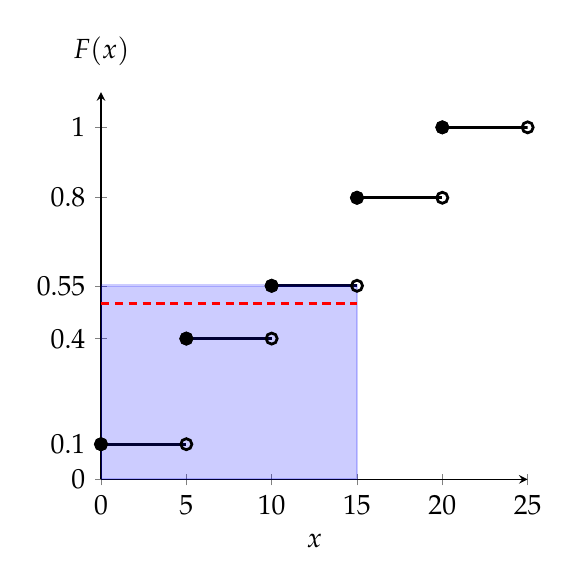
\begin{tikzpicture}
    \begin{axis}[
        height=6.5cm,
        width=7cm,
        axis x line=bottom,
        axis y line=left,
        xlabel = {$x$},
        title = {\hspace*{-5.5cm} $F(x)$},
        ytick={0, 0.10, 0.40, 0.55, 0.80, 1},
        xmin = 0,
        xmax = 25,
        ymin = 0,
        ymax = 1.1]
        \addplot[mark=o, draw=black, line width=1pt] coordinates { (0,0.1)(5,0.1) };
        \addplot[mark=o, draw=black, line width=1pt] coordinates { (5,0.4)(10,0.4) };
        \addplot[mark=o, draw=black, line width=1pt] coordinates { (10,0.55)(15,0.55) };
        \addplot[mark=o, draw=black, line width=1pt] coordinates { (15,0.8)(20,0.8) };
        \addplot[mark=o, draw=black, line width=1pt] coordinates { (20,1)(25,1) };

        \addplot[mark=*, draw=black, line width=1pt] coordinates { (0,0.1) };
        \addplot[mark=*, draw=black, line width=1pt] coordinates { (5,0.4) };
        \addplot[mark=*, draw=black, line width=1pt] coordinates { (10,0.55) };
        \addplot[mark=*, draw=black, line width=1pt] coordinates { (15,0.8) };
        \addplot[mark=*, draw=black, line width=1pt] coordinates { (20,1) };

        \addplot[mark=none, draw=blue, line width=1pt, fill=blue, opacity=0.2] coordinates { (0,0.55)(15,0.55) }\closedcycle;
        \addplot[mark=none, draw=red, line width=1pt, densely dashed] coordinates { (0,0.50)(15,0.50) };

        \draw (45,25) node[right]{$F^{-1}(0.50) = 10$};
    \end{axis}
\end{tikzpicture}

\section*{Contract}
\begin{itemize}[align=left,leftmargin=*]
    \item \textbf{Deductible(d)}
    \item \textbf{Maximum(u)}
    \item \textbf{Inflation(r)}
    \item \textbf{Coinsurance($\boldsymbol{\alpha}$)}
\end{itemize}
\begin{align*}
    Y &= 
    \left\{ 
        \begin{array}{cc}
        0 & x \leq \frac{d}{1+r}\\
        \alpha[(1+r)x-d] & \frac{d}{1+r} < x < \frac{u}{1+r} \\
        \alpha[u - d] & x \geq \frac{u}{1+r} \\
        \end{array}  
    \right.
\end{align*} \\
{\color{red} Warning: The maximal don't include the deductible.}

\section*{Moments}
\begin{itemize}[align=left,leftmargin=*]
    \item k\up{e} moment about the origin. $\mu_k'=\esp{X^k}$
    \item k\up{e} moment about the mean. $\mu_k=\esp{(X-\mu)^k}$
    \item The \textbf{Skewness} moment give infomation about the asymmetry of the distribution. If $S_{sk}=0$, the distribution is normal. \[\hspace*{1cm} S_{sk} = \esp{\left(\frac{X-\mu}{\sigma^2}\right)^3} \] %If $S_{sk}=0$, the distribution is normal.
    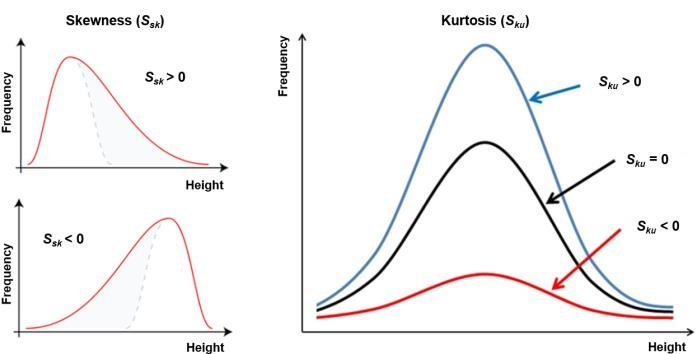
\includegraphics[scale=0.34]{src/Illustration-skewness-and-kurtosis.png}
    \item The \textbf{kurtosis} moment give infomation about the flattening of the distribution. If $S_{ku}=0$, the distribution is normal. \[\hspace*{1cm} S_{ku} = \esp{\left(\frac{X-\mu}{\sigma^2}\right)^4} \] %If $S_{ku}=0$, the distribution is normal.
    \item The \textbf{coefficient of variation} give information about the dispersion of the distribution. \[\hspace*{1.1cm} \mathrm{CV} = \frac{\sigma}{\esp{X}} \]
\end{itemize}

\section*{Transformations of distribution}
\label{Appendix: Transformations distribution}
\begin{itemize}[align=left,leftmargin=*]
    \item Lognormal: $Y = e^{X}$, where
    \begin{align*}
        Y &\sim \mathrm{Lognormal}(\mu, \sigma) \\
        X &\sim \mathrm{Normal}(\mu, \sigma)
    \end{align*}
    \item Inverse Exponential: $Y = \frac{1}{X}$, where 
    \begin{align*}
        Y &\sim \mathrm{Inverse\:Exponential}(1/\theta) \\
        X &\sim \mathrm{Exponential}(\theta)
    \end{align*}
    \item Weibull: $Y = X^{1/\tau}$, where
    \begin{align*}
        Y &\sim \mathrm{Weibull}(\sqrt[\tau]{\theta}) \\
        X &\sim \mathrm{Exponential}(\theta)
    \end{align*}
\end{itemize}

\section*{Parameter interpretation}
\begin{itemize}[align=left,leftmargin=*]
    \item \textbf{Scale parameter ($\theta$, $\beta$, $\sigma$):} Affect the spread of the distribution.
    \item \textbf{Rate parameter ($\lambda$):} Affect the rate of data at mean. (1/scale)
    \item \textbf{Shape parameter ($\alpha$, $\tau$, $\gamma$):} Affect the shape rather then simply shift the distribution.
\end{itemize}

\end{multicols*}
%% -----------------------------
%% Fin du document
%% -----------------------------
\end{document}